La simulation ne doit s’arrêter que quand on la quitte. On sait donc déjà qu’il y aura une boucle
presque infinie au centre du programme, afin d’éxécuter chaque action qui fait partie d’un cycle de
simulation. On peut donc imaginer une boucle principale de cette manière : 
\begin{figure}[H]
	\centering
	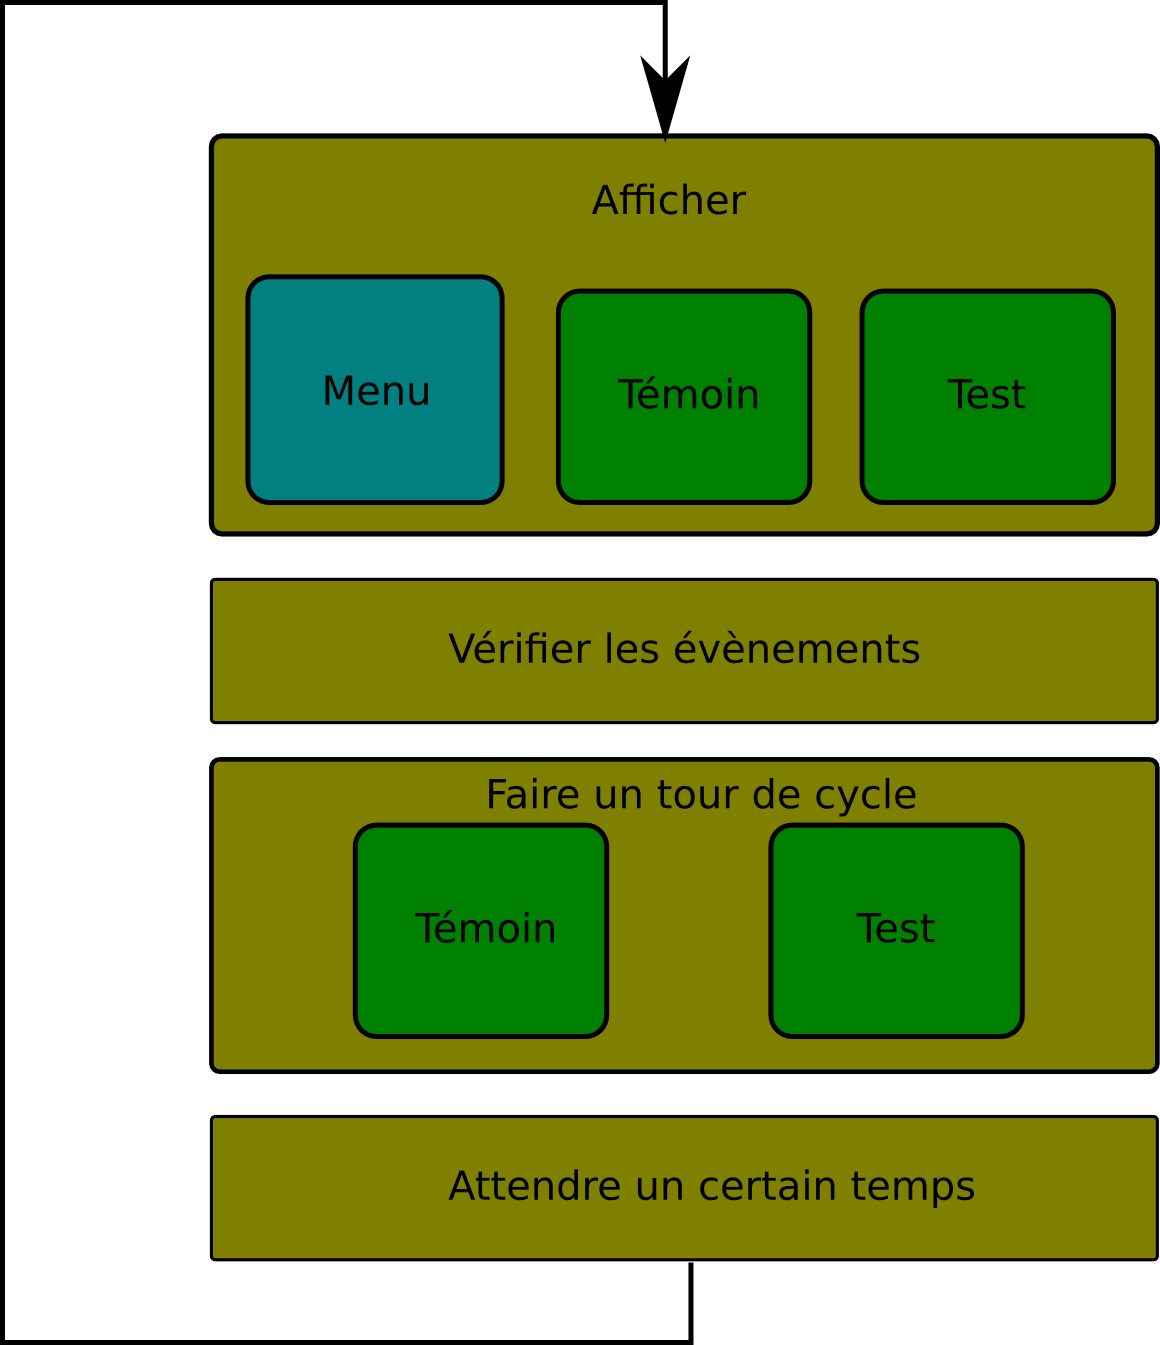
\includegraphics[width=26em]{Images/boucle_naive.png}
	\caption{Une première idée de boucle}
\end{figure}

\begin{description}
	\item[Afficher] : Dessiner le menu, la simulation témoin, la simulation test, et tout ce qu'ils contiennent sur l'écran
	\item[Vérifier les évènements] : récupérer le premier évènement produit et le traiter
	\item[Faire un tour de cycle] : exécuter\footnote{C'est un terme volontairement vague, à ce stade, on ne sait pas encore exactement ce que la simulation va faire} un tour de cycle pour la simulation témoin et la simulation test
	\item[Attendre] : Pour que la simulation soit plus constante, sans cela elle ira aussi vite que possible, et donc sera irrégulière en fonction de la densité de calcul
	\item[Recommencer] : jusqu'à ce que l'on ai demandé de quitter (géré dans les évènements)
\end{description}

On peut imaginer une vision moins naive de cette boucle en divisant les différentes actions en différents processus distincts. Cette méthode est très utile car les processus s'exécutent en parallèle ou presque\footnote{C'est le système d'exploitation qui se charge de leur répartir du temps de calcul, ils ne sont donc pas vraiment en parallèle, sauf avec les ordinateurs récents qui ont plusieurs unités de calcul (processeurs)}. Ceci permet d'avoir une 
vitesse d'affichage constante, par exemple 30 images par secondes, une vitesse d'exécution des simulation différente et une boucle qui gère les évènements avec une vitesse encore différente.

\begin{figure}[H]
	\centering
	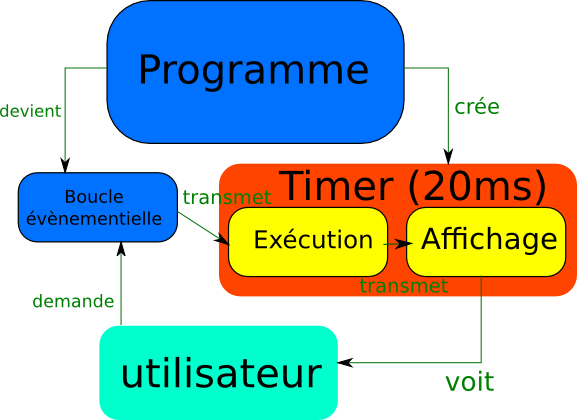
\includegraphics[width=26em]{Images/fonctionnement_programme.png}
	\caption{Fonctionnement du programme}
\end{figure}

Bien sûr il faut que les processus puissent communiquer entre eux. Et cela pose problème, étant donné qu'ils s'exécutent en parallèle, et qu'on ne sait pas lequel va être lancé en premier. On peut leur faire partager des variables, mais il faut bien vérifier qu'elle soit à jour, et éviter les modifications simultanées par deux processus d'une même variable ! C'est la seule difficulté rencontrée par la séparation en plusieurs processus, la solution a été d'utiliser des verrous : avant de faire une action on demande un verrou sur cette variable et on est sur que personne d'autre que nous ne peut la modifier, ensuite on libère le verrou, et c'est un autre processus qui prend possession de la variable. Cette méthode peut entrainer des ralentissements, des décalages, mais nous ne partageons que 2 variables, donc normalement, il n'y a pas de raisons que ces ralentissements soient visibles.

